% 右手定则

物理中常用右手定则来判断方向, 右手定则分为以下两种.

\begin{figure}[ht]
\centering
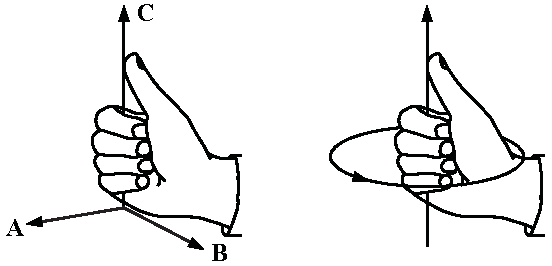
\includegraphics[width=9cm]{./figures/RHRul1.pdf}
\caption{两种右手定则} \label{RHRul_fig1}
\end{figure}

\subsection{第一种右手定则}
假设有两个不共线的矢量, 第一个为 $\vec A$, 第二个为 $\vec B$, 它们可以定义一个平面. 现在我们想根据 $\vec A$ 和 $\vec B$ 确定该平面的法向量 $\vec C$, 但由于平面的法向量有两个, 我们如何区分它们呢? 我们可以通过\autoref{RHRul_fig1} (左) 所示的右手定则来确定其中一个法向量: 首先将右手的四指指向 $\vec A$, 再将四指弯向 $\vec B$, 这时伸出拇指, 拇指的方向即为右手定则定义的方向.

我们通常使用的空间直角坐标系被称为“右手系”, 是因为我们可以通过右手定则从 $x$ 轴和 $y$ 轴的方向定义 $z$ 轴的方向(\autoref{RHRul_fig2} 右). 同理, 我们也可以定义所谓的“左手系”.

\begin{figure}[ht]
\centering
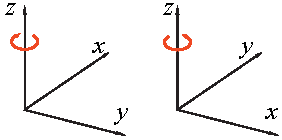
\includegraphics[width=6cm]{./figures/RHRul2.pdf}
\caption{左手系(左)与右手系(右)} \label{RHRul_fig2}
\end{figure}

\subsection{第二种右手定则}
假设空间中有一圆环, 且圆环上有一正方向, 我们可以用右手定则指定圆环所在平面的一个法向量.如\autoref{RHRul_fig1}(右), 用右手握住该圆环, 手指与圆环平行, 且指尖指向圆环的正方向, 伸出拇指, 则拇指所指的方向就是右手定则判断的方向.
